\chapter{Introdução}

\section{Ensaio de Fluxo no Cabeçote}

Um motor de combustão interna é uma máquina que converte a energia química em energia cinética. 
Sua evolução teve início com o desenvolvimento das máquinas térmicas a vapor no século XVIII. 
Em 1862, Nicolaus Otto patenteou o motor de ciclo Otto e, em 1892, Rudolf Diesel patenteou o primeiro motor de ignição por compressão.
Desde então, essas máquinas térmicas têm passado por um processo contínuo de aprimoramento, para oferecer maior versatilidade de operação e maior eficiência térmica. 
Isso é realizado para reduzir as emissões de poluentes na atmosfera e melhorar o desempenho dos motores. 
Atualmente, uma tecnologia amplamente empregada em motores de combustão interna que operam no ciclo Otto é o VVT (Variable Valve Timing), que envolve o ajuste da abertura das válvulas e do perfil do comando de válvulas.

O cabeçote é uma parte fundamental do motor, pois cobre os cilindros e aloja vários componentes. 
Sua principal função é garantir uma vedação perfeita com o bloco do motor, suportando as altas temperaturas e pressões geradas durante a combustão nos cilindros. 
Para cumprir esta função, o cabeçote utiliza uma junta de vedação feita de material metálico, capaz de compensar pequenas irregularidades nas superfícies do bloco e do próprio cabeçote, garantindo uma vedação completa. 
A fixação do cabeçote ao bloco é feita com parafusos de alta resistência e dureza, criando uma pressão de contato entre as superfícies do bloco e do cabeçote maior do que a pressão na câmara de combustão. 
Isso é essencial para evitar vazamentos de gases e líquidos, bem como a contaminação entre as partes internas do motor. Garantir a correta fixação do cabeçote é crucial para o funcionamento eficaz e duradouro do motor.

A bancada de fluxo é um equipamento amplamente utilizado por indústrias e laboratórios para realizar testes de vazão nas válvulas dos motores de combustão interna. 
Esse equipamento mede o fluxo de ar através das válvulas com base na diferença de pressão gerada. 
Ele é composto por um conjunto de tubulações, válvulas, bombas e medidores de vazão. 
Quando acoplado ao cabeçote do motor usado nos testes, a bancada fornece dados importantes para a análise do motor, como a queda de pressão nas válvulas e a vazão através delas. 
Um exemplo de uma bancada de fluxo fabricada pela SERVITEC pode ser observado na~\cref{fig:bancada_fluxo}.
%
\begin{figure}[!htb]
    \centering
    \caption{Bancada de Fluxo}
    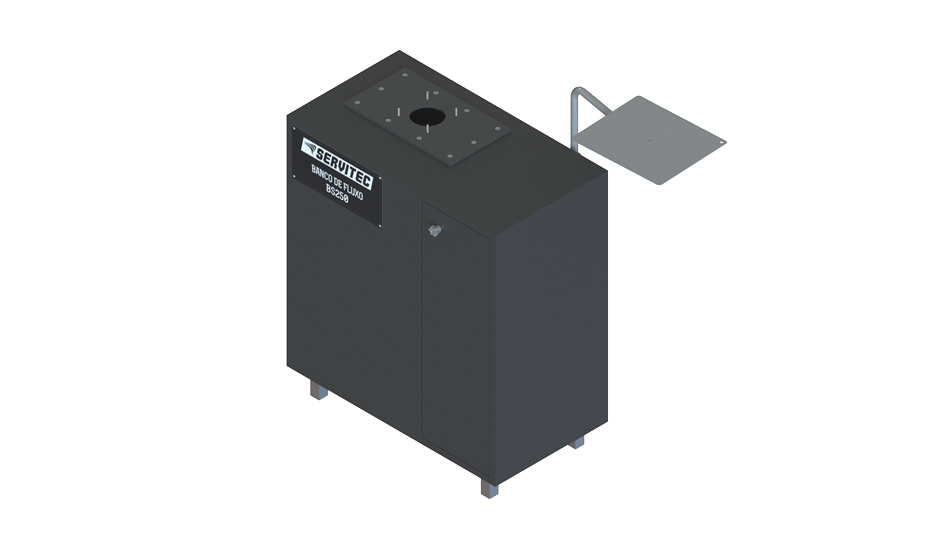
\includegraphics[width=0.8\textwidth]{figuras/banca_fluxo.png}
    \fonte{\url{https://www.servitecdinamometro.com.br/produto/modelo-bs250}}
    \label{fig:bancada_fluxo}
\end{figure}
%
No experimento, foi empregado o cabeçote do motor EA211 1.0 TSI, de origem alemã e fabricado no Brasil pela Volkswagen. 
Este cabeçote é utilizado em quatro veículos que se apresentam em três configurações distintas: o Up! TSI, Golf Comfortline, Polo 200 TSI e Virtus 200 TSI. 
Para conduzir o experimento na bancada de fluxo, foram necessárias algumas modificações no cabeçote. Isso incluiu a adaptação do mecanismo de controle das válvulas de admissão e escape, permitindo o ajuste da abertura das válvulas, e a incorporação de um acoplamento tipo corneta na entrada de admissão, seguindo as diretrizes da norma ABNT NBR ISO 5167. 
Isso foi feito com o objetivo de minimizar o efeito de vena contracta, resultando em um fluxo uniforme na entrada do duto de admissão, conforme ilustrado na~\cref{fig:acoplamento}.
%
\begin{figure}[!htb]
    \centering
    \caption{Acoplamento}
    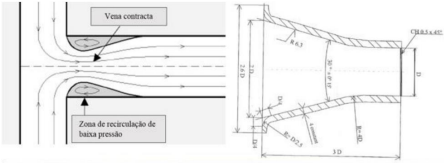
\includegraphics[width=0.7\textwidth]{figuras/acoplamento.png}
    \fonte{ }
    \label{fig:acoplamento}
\end{figure}
%
No experimento, foi empregada a bancada de modelo BS400X, e as especificações técnicas detalhadas estão fornecidas na~\cref{tab:especificacoes_bancada}.
%
\begin{table}[!htb]
    \centering
    \caption{Informações técnicas da bancada de fluxo}
    \begin{tblr}{
        row{even} = azul!10,
        colspec = {*{2}{X[l]}}
    }
    \toprule
    Parâmetros & Valor \\
    \midrule
    Capacidade de sucção & 420 cfm a 10 in\ce{H2O} 390 cfm a 28 in\ce{H2O} \\
    Capacidade de exaustão & 420 cfm à 10 in\ce{H2O} 390 cfm à 28 in\ce{H2O} \\
    Diferença máxima de pressão & 40 in\ce{H2O} \\
    Medição de fluxo & cfm ou L/s \\
    Medição de pressão de teste & in\ce{H2O}, kPa, psi, $\mu$bar \\
    \bottomrule
    \end{tblr}
    \fonte{\url{https://www.servitecdinamometro.com.br/produto/modelo-bs250}}
    \label{tab:especificacoes_bancada}
\end{table}
%
\section{Ensaio Dinamométrico}

Sendo um motor de combustão interna uma máquina complexa, com diversos componentes funcionando em sintonia simultaneamente.
É produzido em larga escala para atender a demanda por geradores de energia para máquinas automotivas, e dever ser garantido seu funcionamento em diversas configurações e condições de operação. 
O dinamômetro é um aparelho com o objetivo de medir cargas como força e torque, mas pela configuração geral do sistema, pode-se aferir rotação, potência e temperatura. 
Por isso, seu uso é imprescindível no teste de novos projetos, correções e manutenções de motores.

A~\cref{fig:dinamometro} mostra um dinamômetro, com a estrutura em amarelo compondo o dinamômetro e célula de carga, o pilar branco contendo um trocador de calor para manter a água do dinamômetro em temperatura de funcionamento e a caixa preta contém o maquinário de bombas hidráulicas.
%
\begin{figure}[!htb]
    \centering
    \caption{Dinamômetro}
    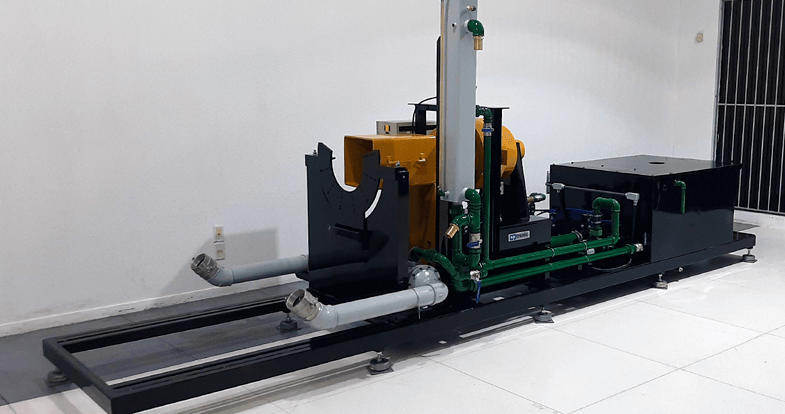
\includegraphics[width=0.7\textwidth]{figuras/dinamometro.png}
    \fonte{\url{https://girotti.com.br/dinamometro-de-motores/}}
    \label{fig:dinamometro}
\end{figure}
%
O principal objetivo ao usar este aparelho é verificar os efeitos da mudança de múltiplos parâmetros, que simulem as variações no mundo real como: mudança no combustível, vazão de ar, rotação, carga no motor e com isso avaliar seu desempenho, para então propor modificações e soluções que possam ser produtivas.

O dinamômetro hidráulico é composto por um estator de metal com um rotor imerso em óleo e a medida que o eixo do motor gira, o rotor interage com o fluido que resiste ao movimento, gerando calor por meio de atrito viscoso. Ele também produz força de atrito no rotor, o qual atua como carga para o motor, como mosta a~\cref{fig:dinamometro_funcionamento}. 
%
\begin{figure}[!htb]
    \centering
    \caption{Funcionamento do Dinamômetro}
    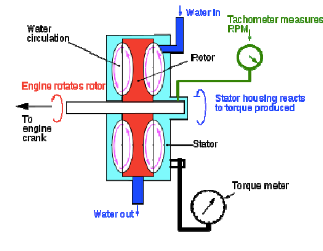
\includegraphics[width=0.7\textwidth]{figuras/dinamometro_funcionamento.png}
    \fonte{https://mechdiploma.com/?q=node/219}
    \label{fig:dinamometro_funcionamento}
\end{figure}
%
\section{Objetivos}

O presente relatório tem como objetivo realizar uma análise entre dois experimentos distintos: o ensaio de fluxo realizado em um cabeçote do motor EA211 TSI e o desempenho do motor diesel da marca John Deere. O objetivo é fornecer uma avaliação abrangente das características de fluxo e eficiência destes dois motores, abordando aspectos relevantes para a otimização do desempenho e eficiência energética. 



